\documentclass[11pt]{article}

\usepackage[margin=1in]{geometry}
\usepackage{amsmath,amssymb,amsthm,mathtools}
\usepackage{graphicx}
\usepackage{hyperref}
\usepackage{enumitem}
\usepackage{microtype}

\title{Graphs as Construction Histories: A Mixed-Radix Bijection via Matula Trees}
\author{William Matula}
\date{\today}

\newtheorem{theorem}{Theorem}
\newtheorem{lemma}{Lemma}
\newtheorem{definition}{Definition}
\newtheorem{proposition}{Proposition}

\graphicspath{{../figures/}}

\begin{document}
\maketitle

\begin{abstract}
We present a bijection between finite unlabeled graphs and integers based on
vertex-by-vertex construction histories encoded in a mixed-radix system. The
canonical representative is defined as the minimum mixed-radix integer over all
labelings, yielding a global ordering that emphasizes build complexity rather
than adjacency sparsity. The construction integer is itself a Matula number,
providing an explicit rooted-tree interpretation. We compare this construction
bijection with canonical adjacency, product invariants, and a block-cut
``red-node'' encoding, and we outline qualitative stress tests that distinguish
these orderings on small graphs.
\end{abstract}

\section{Introduction}
Matula's bijection between rooted trees and integers gives a concrete way to
read arithmetic structure as combinatorial structure. Extending this idea from
rooted trees to general graphs raises two constraints: a canonical choice over
labelings and a representation with interpretable structure. We propose a
construction-based encoding that treats graphs as histories of incremental
vertex additions.

\paragraph{Contributions.}
\begin{enumerate}[label=\arabic*.]
    \item A mixed-radix encoding of construction sequences that yields a bijection
    between graphs and integers once canonicalized by minimum integer.
    \item A Matula-tree interpretation of each construction integer, yielding a
    structural diagram for the construction grammar.
    \item A comparison framework that contrasts this ordering with canonical
    adjacency, product invariants, and block-cut (red-node) encodings.
\end{enumerate}

\section{Preliminaries}
\subsection{Graphs and labelings}
All graphs are finite, undirected, and simple. For a graph on $n$ vertices,
consider all $n!$ labelings; canonicalization requires selecting a unique
representative among these labelings.

\subsection{Matula numbers}
Matula's bijection maps rooted trees to integers via prime factorization
\cite{matula1968,goebel1980}. We assume the standard definitions; this paper
uses the fact that any nonnegative integer corresponds to a unique rooted tree.

\section{Construction sequences and mixed-radix encoding}
\begin{definition}[Construction sequence]
Fix a labeling of a graph with vertices ordered as $v_0, v_1, \dots, v_{n-1}$.
For each $k \ge 1$, let $c_k \in \{0,1,\dots,2^k-1\}$ be the bitmask indicating
which of $v_0,\dots,v_{k-1}$ are adjacent to $v_k$. The sequence
$[c_1,\dots,c_{n-1}]$ is the \emph{construction sequence} for the labeling.
\end{definition}

\begin{definition}[Mixed-radix encoding]
The construction integer is
\[
    \mathrm{C}(G,\pi) = \sum_{k=1}^{n-1} c_k \prod_{j=1}^{k-1} 2^j,
\]
where $\pi$ is the chosen labeling order and the empty product is $1$.
\end{definition}

\begin{definition}[Canonical construction integer]
The canonical construction integer of an unlabeled graph $G$ is
\[\mathrm{C}(G) = \min_{\pi} \mathrm{C}(G,\pi),\]
where $\pi$ ranges over all labelings.
\end{definition}

\begin{proposition}
For fixed $n$, the mapping from construction sequences to integers is a bijection.
\end{proposition}

\begin{theorem}[Canonical construction bijection]
For each unlabeled graph $G$, the canonical construction integer $\mathrm{C}(G)$
is well-defined and unique. The mapping that sends $G$ to $\mathrm{C}(G)$ is
injective on unlabeled graphs, and the mixed-radix encoding provides a decoding
from integers to construction sequences for each fixed $n$.
\end{theorem}

\paragraph{Proof sketch.}
For fixed $n$, the mixed-radix encoding is a bijection between sequences
$[c_1,\dots,c_{n-1}]$ and integers in $[0,\prod_{k=1}^{n-1}2^k)$, so decoding is
unique. For any unlabeled graph $G$, the set of labelings is finite, so the
minimum construction integer exists. If two graphs had the same canonical
integer, then they would share a construction sequence under some labeling,
which determines the adjacency pattern and hence the isomorphism class.

\section{Matula trees for construction integers}
Because each construction integer is a nonnegative integer, it corresponds to a
unique rooted tree under the Matula bijection. This yields a compositional tree
diagram for the construction grammar of the graph (see Fig.~4).

\section{Comparisons and stress tests}
We contrast the construction bijection with three alternatives:
canonical adjacency encoding, product invariants over all labelings, and a
block-cut red-node encoding. We emphasize examples where the orderings diverge
(e.g., star vs path in Fig.~1, cycle vs matching in Fig.~2, and barbell vs two
triangles in Fig.~3).

\paragraph{Small $n=5$ example list.}
Ordering the unlabeled graphs by canonical adjacency and listing the resulting
construction integers for $n=5$ gives:
\[
0, 1, 3, 11, 75, 7, 12, 13, 15, 76, 77, 79, 30, 31, 86, 87, 94, 95, 222, 223, 63, 116, 117, 119, 127, 235, 236, 237, 239, 254, 255, 507, 511, 1023.
\]

\begin{figure}[h]
    \centering
    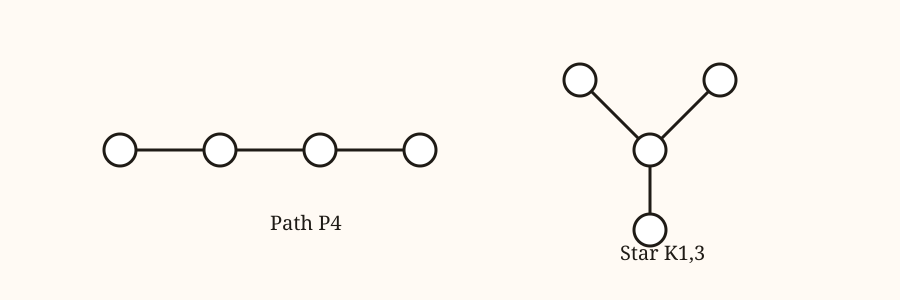
\includegraphics[width=\linewidth]{path-star.svg}
    \caption{Path vs star: same size, different construction profiles.}
\end{figure}

\begin{figure}[h]
    \centering
    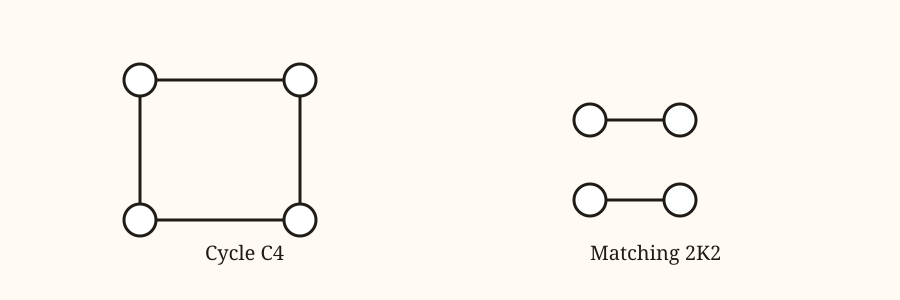
\includegraphics[width=\linewidth]{cycle-matching.svg}
    \caption{Cycle vs matching: same $n$ and $m$, different symmetry profiles.}
\end{figure}

\begin{figure}[h]
    \centering
    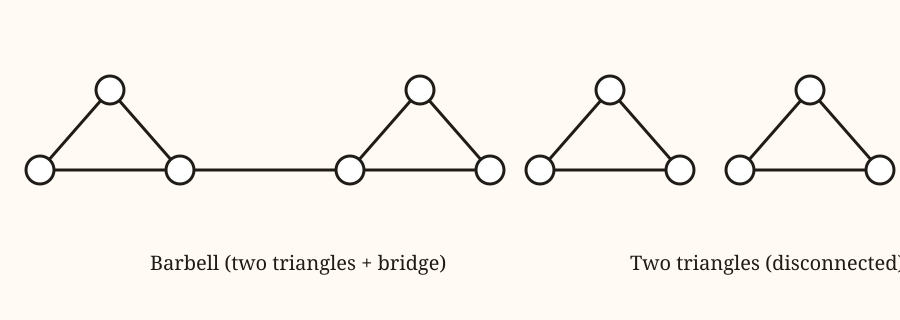
\includegraphics[width=\linewidth]{barbell-two-triangles.svg}
    \caption{Barbell vs two disconnected triangles: same blocks, different topology.}
\end{figure}

\begin{figure}[h]
    \centering
    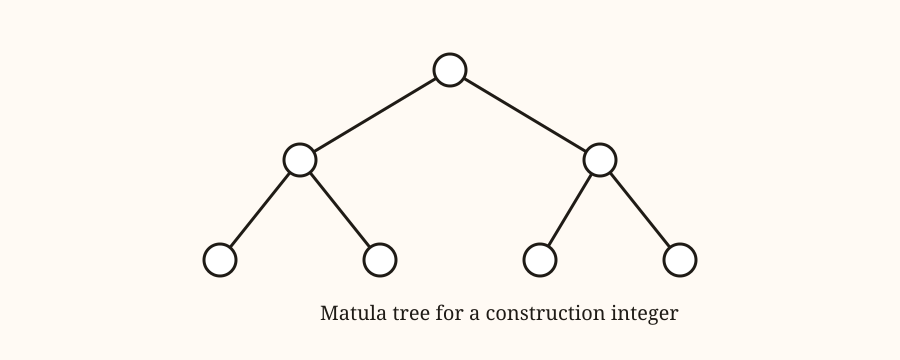
\includegraphics[width=0.8\linewidth]{matula-tree.svg}
    \caption{A Matula tree diagram for a construction integer.}
\end{figure}

\section{Complexity and canonicalization}
Canonical construction requires considering all $n!$ labelings in the worst
case, matching the known hardness of graph canonicalization. The contribution is
structural, not algorithmic: the ordering makes constructional complexity
visible rather than hidden. For practical canonical labeling algorithms, see
the nauty/traces line of work \cite{mckay2014}.

\section{Related work}
Canonical adjacency encodings of unlabeled graphs appear in the literature as
``mincode'' or graph-code numbers: one minimizes the lower-triangular adjacency
bitstring over all labelings and interprets it as an integer
\cite{harary1970,parthasarathy2002}. OEIS sequences A076184 and A382754
enumerate these canonical adjacency codes, and A382757 maps the corresponding
graph list to those codes. Our work differs in the encoding semantics: the
integer is derived from a construction history (mixed-radix sequence) and then
decoded as a Matula tree, which supplies a compositional interpretation beyond
canonical adjacency.

\section{Discussion and open questions}
We outline possible correlations between construction complexity and classical
graph invariants, and ask whether block-cut decomposition can be combined with
construction encoding to reduce collisions while preserving structure.

\bibliographystyle{plain}
\bibliography{references}

\end{document}
